
%%%%%%%%%%%%%%%%%%%%%%%%%%%%%%%%%%%%%%%%%%%%%%%%%%%%%%%%%%%%%%%%%%%%%%%%%%%%%%%%%%
\begin{frame}[fragile]\frametitle{}
\begin{center}
{\Large Generic Applications of Prompts}
\end{center}
\end{frame}


%%%%%%%%%%%%%%%%%%%%%%%%%%%%%%%%%%%%%%%%%%%%%%%%%%%%%%%%%%%%%%%%%%%%%%%%%%%%%%%%%%
\begin{frame}[fragile]\frametitle{Explain Complex Subjects}
\begin{center}
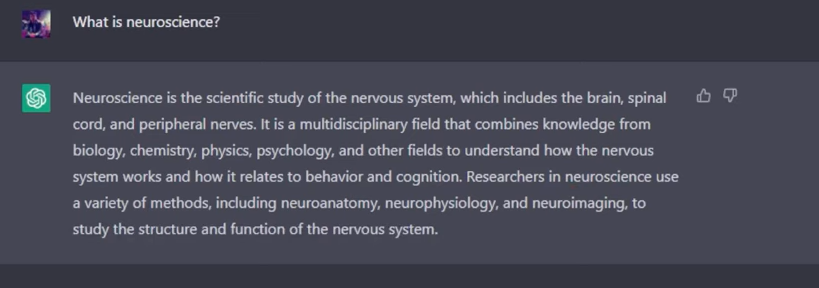
\includegraphics[width=\linewidth,keepaspectratio]{chatgpt15}
\end{center}
	
{\tiny (Ref: Top 10 Chat GPT Use Cases - Simplilearn)}
\end{frame}

%%%%%%%%%%%%%%%%%%%%%%%%%%%%%%%%%%%%%%%%%%%%%%%%%%%%%%%%%%%%%%%%%%%%%%%%%%%%%%%%%%
\begin{frame}[fragile]\frametitle{Write Code}
\begin{center}
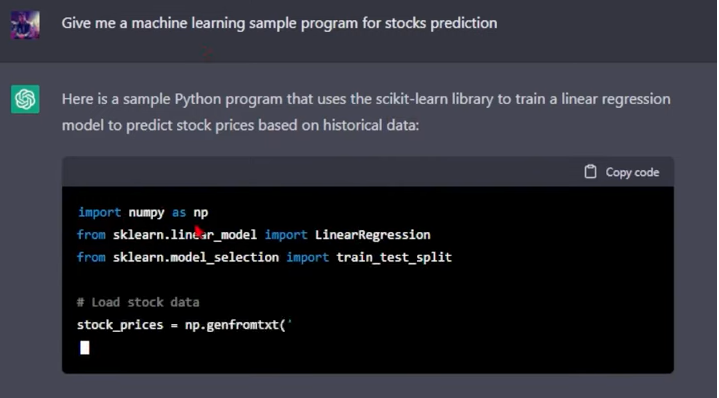
\includegraphics[width=0.8\linewidth,keepaspectratio]{chatgpt16}
\end{center}

it was still writing but I stopped it, just to show this pic

{\tiny (Ref: Top 10 Chat GPT Use Cases - Simplilearn)}
\end{frame}

%%%%%%%%%%%%%%%%%%%%%%%%%%%%%%%%%%%%%%%%%%%%%%%%%%%%%%%%%%%%%%%%%%%%%%%%%%%%%%%%%%
\begin{frame}[fragile]\frametitle{Debug Code}
\begin{center}
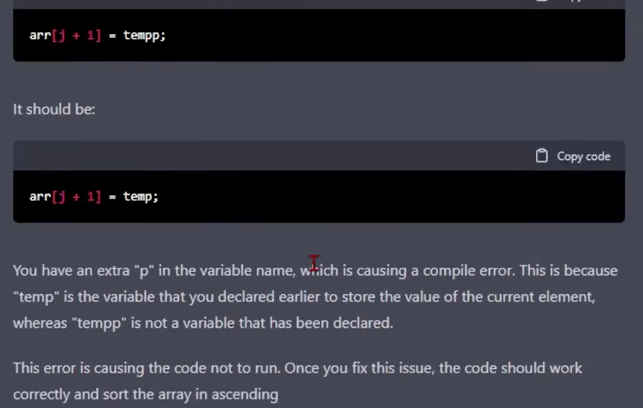
\includegraphics[width=0.8\linewidth,keepaspectratio]{chatgpt17}
\end{center}

{\tiny (Ref: Top 10 Chat GPT Use Cases - Simplilearn)}
\end{frame}

%%%%%%%%%%%%%%%%%%%%%%%%%%%%%%%%%%%%%%%%%%%%%%%%%%%%%%%%%%%%%%%%%%%%%%%%%%%%%%%%%%
\begin{frame}[fragile]\frametitle{Get Custom Marketing Strategy}
\begin{center}

\includegraphics[width=\linewidth,keepaspectratio]{chatgpt18}
\end{center}

{\tiny (Ref: Top 10 Chat GPT Use Cases - Simplilearn)}
\end{frame}

%%%%%%%%%%%%%%%%%%%%%%%%%%%%%%%%%%%%%%%%%%%%%%%%%%%%%%%%%%%%%%%%%%%%%%%%%%%%%%%%%%
\begin{frame}[fragile]\frametitle{Write Articles}
\begin{center}
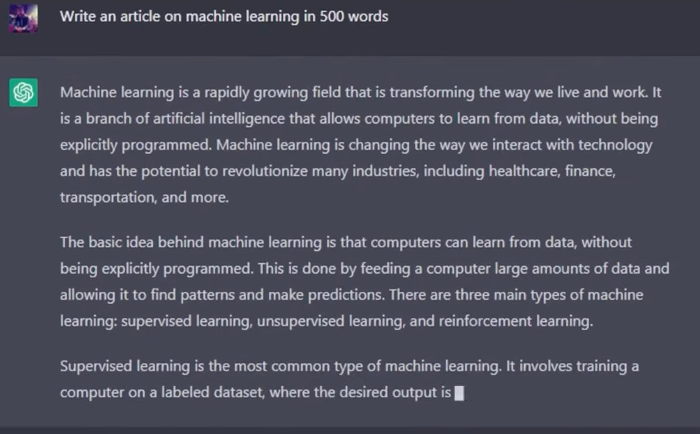
\includegraphics[width=\linewidth,keepaspectratio]{chatgpt19}
\end{center}

{\tiny (Ref: Top 10 Chat GPT Use Cases - Simplilearn)}
\end{frame}

%%%%%%%%%%%%%%%%%%%%%%%%%%%%%%%%%%%%%%%%%%%%%%%%%%%%%%%%%%%%%%%%%%%%%%%%%%%%%%%%%%
\begin{frame}[fragile]\frametitle{Summarize Book}
\begin{center}
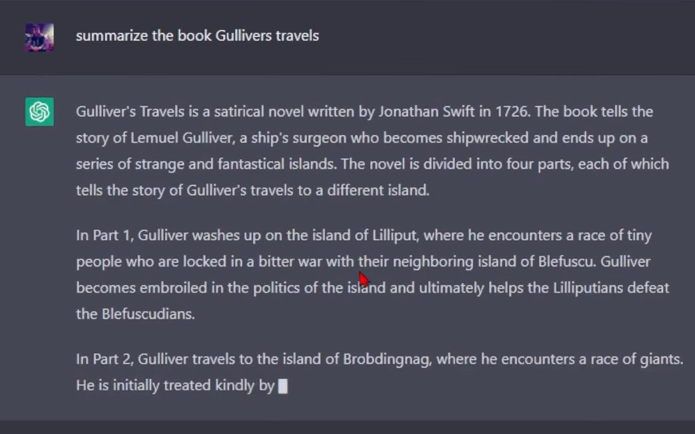
\includegraphics[width=\linewidth,keepaspectratio]{chatgpt20}
\end{center}

{\tiny (Ref: Top 10 Chat GPT Use Cases - Simplilearn)}
\end{frame}

%%%%%%%%%%%%%%%%%%%%%%%%%%%%%%%%%%%%%%%%%%%%%%%%%%%%%%%%%%%%%%%%%%%%%%%%%%%%%%%%%%
\begin{frame}[fragile]\frametitle{Answer Interview Questions}
\begin{center}
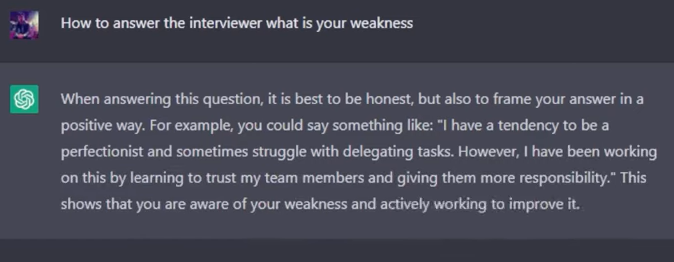
\includegraphics[width=\linewidth,keepaspectratio]{chatgpt21}
\end{center}

{\tiny (Ref: Top 10 Chat GPT Use Cases - Simplilearn)}
\end{frame}



%%%%%%%%%%%%%%%%%%%%%%%%%%%%%%%%%%%%%%%%%%%%%%%%%%%%%%%%%%%%%%%%%%%%%%%%%%%%%%%%%%
\begin{frame}[fragile]\frametitle{Develop Apps}
\begin{center}
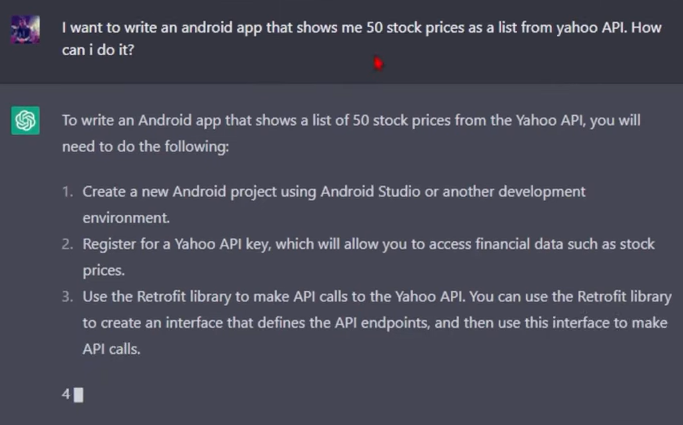
\includegraphics[width=\linewidth,keepaspectratio]{chatgpt22}
\end{center}

{\tiny (Ref: Top 10 Chat GPT Use Cases - Simplilearn)}
\end{frame}

%%%%%%%%%%%%%%%%%%%%%%%%%%%%%%%%%%%%%%%%%%%%%%%%%%%%%%%%%%%%%%%%%%%%%%%%%%%%%%%%%%
\begin{frame}[fragile]\frametitle{Create Health Plan}
\begin{center}
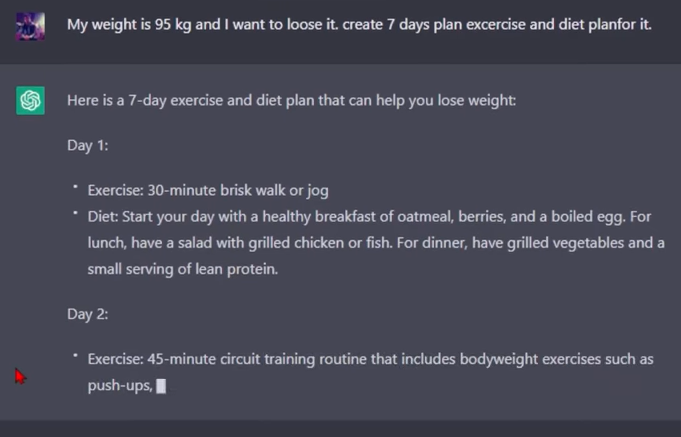
\includegraphics[width=\linewidth,keepaspectratio]{chatgpt23}
\end{center}

{\tiny (Ref: Top 10 Chat GPT Use Cases - Simplilearn)}
\end{frame}

%%%%%%%%%%%%%%%%%%%%%%%%%%%%%%%%%%%%%%%%%%%%%%%%%%%%%%%%%%%%%%%%%%%%%%%%%%%%%%%%%%
\begin{frame}[fragile]\frametitle{Answer General Knowledge Questions}
\begin{center}
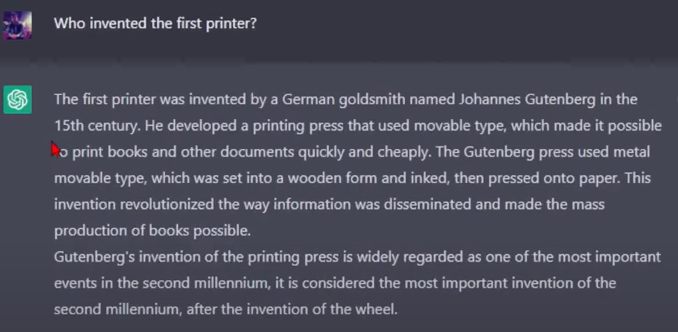
\includegraphics[width=\linewidth,keepaspectratio]{chatgpt24}
\end{center}

{\tiny (Ref: Top 10 Chat GPT Use Cases - Simplilearn)}
\end{frame}


%%%%%%%%%%%%%%%%%%%%%%%%%%%%%%%%%%%%%%%%%%%%%%%%%%%%%%%%%%%%%%%%%%%%%%%%%%%%%%%%%%
\begin{frame}[fragile]\frametitle{Advanced Prompts}
\begin{itemize}
    \item  Five Whys Technique: ``Act like a Root Cause Analyst. Begin by identifying the problem related to [topic]. Now, ask 'why?' this problem exists. Repeat the question 'why?' four more times, digging deeper into each layer to uncover the root cause. Summarize your findings and suggest potential solutions.''
	\item TRIZ (Theory of Inventive Problem Solving): "Act like an Inventive Problem Solver. Utilize TRIZ principles to systematically solve problems related to [topic]. Identify contradictions and apply inventive principles to resolve them. Outline your steps and findings, explaining how the TRIZ methodology was applied."
	\item Job-To-Be-Done Framework: "Act like a Customer Insight Specialist. Examine [topic] through the Job-To-Be-Done lens, exploring the underlying 'jobs' customers are 'hiring' the product or service to accomplish. Detail the customer needs, contexts, and pain points. Propose alignment strategies to meet these 'jobs.'"
	\item Ishikawa Diagram (Fishbone Diagram): "Act like a Quality Improvement Specialist. Build an Ishikawa diagram to explore the causes of a problem related to [topic]. Break down each main branch into finer details, exploring root causes and relationships. Provide insights into potential solutions and preventive measures."
\end{itemize}

{\tiny (Ref: LinkedIn Post - Ruben Hassid)}
\end{frame}

%%%%%%%%%%%%%%%%%%%%%%%%%%%%%%%%%%%%%%%%%%%%%%%%%%%%%%%%%%%%%%%%%%%%%%%%%%%%%%%%%%
\begin{frame}[fragile]\frametitle{Advanced Prompts}
\begin{itemize}
    \item Zwicky Box (Morphological Analysis): "Act like a Complex Systems Analyst. Utilize a Zwicky Box to systematically explore all possible solutions for [topic]. Define dimensions, attributes, and interactions within the system. Explain how you developed the combinations and their relevance to [topic]."
    \item Affinity Diagram: "Act like an Organizational Psychologist. Organize ideas related to [topic] into an affinity diagram. Group concepts by natural relationships, providing explanations for each category. Analyze the groupings and how they provide a coherent understanding of [topic]."
    \item Ansoff Matrix: "Act like a Growth Strategist. Utilize the Ansoff Matrix to explore growth strategies for [topic]. Assess opportunities for market penetration, market development, product development, and diversification. Explain the rationale for each strategy and propose an implementation plan."
    \item Impact/Effort Matrix: "Act like a Project Management Expert. Plot ideas related to [topic] on an impact/effort matrix. Analyze the strategies that should be prioritized, considering both their potential impact and required effort. Provide a systematic plan for execution, including risk assessment."
\end{itemize}

{\tiny (Ref: LinkedIn Post - Ruben Hassid)}
\end{frame}

% %%%%%%%%%%%%%%%%%%%%%%%%%%%%%%%%%%%%%%%%%%%%%%%%%%%%%%%%%%%%%%%%%%%%%%%%%%%%%%%%%%
% \begin{frame}[fragile]\frametitle{HVAC QnA}
% Prompt: ``Diagnose a frosted evaporator coil''

% Result: 
% ``There are several reasons why an evaporator coil may become frosted:
% \begin{itemize}
% \item Low refrigerant levels: If the refrigerant levels in the system are too low, it can cause the
% evaporator coil to freeze. This is because the refrigerant is responsible for absorbing heat
% from the air, and without enough refrigerant, the coil will not be able to absorb enough heat
% to prevent freezing.
% \item Dirty air filter: A dirty air filter can restrict airflow to the evaporator coil, causing the coil
% to freeze.
% \item Blocked or restricted airflow: If the airflow to the evaporator coil is blocked or
% restricted, the coil may freeze. This can be caused by a number of things such as dirty ducts or
% registers, closed or blocked vents, or a malfunctioning blower fan.
% \item Obstruction in the drain line: A blockage in the drain line can cause water to back up and freeze on the coil.
% \end{itemize}	 
% It's important to fix the issue as soon as possible, as a frozen evaporator coil can lead to decreased
% efficiency and can cause damage to the unit.
% ''

% \tiny{(Ref:ChatGPT Could Be the 'Write' Choice for HVACR Contractors - Joanna R. Turpin)}
% \end{frame}

% %%%%%%%%%%%%%%%%%%%%%%%%%%%%%%%%%%%%%%%%%%%%%%%%%%%%%%%%%%%%%%%%%%%%%%%%%%%%%%%%%%
% \begin{frame}[fragile]\frametitle{HVAC QnA}
% Prompt: ``How to respond to a customer who thinks an air conditioner is
% too expensive''

% Result: ``
% \begin{itemize}
% \item Understand their concerns: Find out why they think the air conditioner is too expensive.
% Are they comparing it to a lower-quality unit? Are they on a tight budget? Understanding
% their concerns will help you address them more effectively.
% \item Provide a detailed explanation of the costs: Explain the costs associated with the air
% conditioner, including the cost of the unit, installation, and any additional materials or labor
% that may be required.
% \item Compare costs with the benefits: Explain the benefits of the air conditioner, such as
% energy efficiency, durability, and long-term cost savings. Explain how the cost of the unit may
% be offset by energy savings in the long run.
% \item Offer financing options: If the customer is unable to afford the air conditioner upfront,
% offer financing options that can help them spread the cost over time.

% \end{itemize}	 

% \ldots

% \tiny{(Ref:ChatGPT Could Be the 'Write' Choice for HVACR Contractors - Joanna R. Turpin)}
% \end{frame}

% %%%%%%%%%%%%%%%%%%%%%%%%%%%%%%%%%%%%%%%%%%%%%%%%%%%%%%%%%%%%%%%%%%%%%%%%%%%%%%%%%%
% \begin{frame}[fragile]\frametitle{HVAC QnA}

% \ldots 

% \begin{itemize}
% \item Provide a written estimate: Provide the customer with a detailed, written estimate that
% outlines the costs associated with the air conditioner and the benefits it will provide. This will
% help them make an informed decision.
% \item Provide a guarantee or warranty on the unit: Provide the customer with a guarantee
% or warranty on the unit to give them peace of mind in their investment.
% \item Provide an alternative solution: If the customer cannot afford the recommended
% solution, offer an alternative solution that fits their budget while still meeting their needs.
% \end{itemize}	 
% It's important to be patient, understanding and provide all the information customers need to
% make a decision that best fits their needs and budget.
% ''

% \tiny{(Ref:ChatGPT Could Be the 'Write' Choice for HVACR Contractors - Joanna R. Turpin)}
% \end{frame}

% %%%%%%%%%%%%%%%%%%%%%%%%%%%%%%%%%%%%%%%%%%%%%%%%%%%%%%%%%%%%%%%%%%%%%%%%%%%%%%%%%%
% \begin{frame}[fragile]\frametitle{If This Then That}


% \begin{itemize}
% \item With well designed prompts, one can format output in json (read, key-value pairs)
% \item Parsing via python program, one can trigger Actions. (GPT3 APIs for now)
% \item Whole pipeline can be put in place programmatically, doing any trigger based work (IFTTT - If This Then That)
% \end{itemize}	 


% \tiny{(Ref: ChatGPT for Arduino - MoonPreneur)}
% \end{frame}

% %%%%%%%%%%%%%%%%%%%%%%%%%%%%%%%%%%%%%%%%%%%%%%%%%%%%%%%%%%%%%%%%%%%%%%%%%%%%%%%%%%
% \begin{frame}[fragile]\frametitle{Possible applications}



% \begin{itemize}
% \item Multi-Language Support: ChatGPT’s ability to translate languages can be combined with Arduino to create multi-language support for devices. This feature makes it possible for users from different countries to interact with the device in their language. For example, you can create a device that provides information about local tourist attractions and supports multiple languages.
% \item Home Automation: One unique application of this combination is in the field of home automation. With ChatGPT’s ability to understand and respond to natural language and the versatility of the Arduino platform, it’s possible to create a fully voice-controlled smart home system. 
% \end{itemize}	 



% \tiny{(Ref: ChatGPT for Arduino - MoonPreneur)}
% \end{frame}

%%%%%%%%%%%%%%%%%%%%%%%%%%%%%%%%%%%%%%%%%%%%%%%%%%%%%%%%%%%%%%%%%%%%%%%%%%%%%%%%%%
\begin{frame}[fragile]\frametitle{}
\begin{center}
{\Large NLP Applications of Prompts}
\end{center}
\end{frame}


%%%%%%%%%%%%%%%%%%%%%%%%%%%%%%%%%%%%%%%%%%%%%%%%%%%%%%%%%%%
\begin{frame}[fragile]\frametitle{Text Generation}

\begin{center}
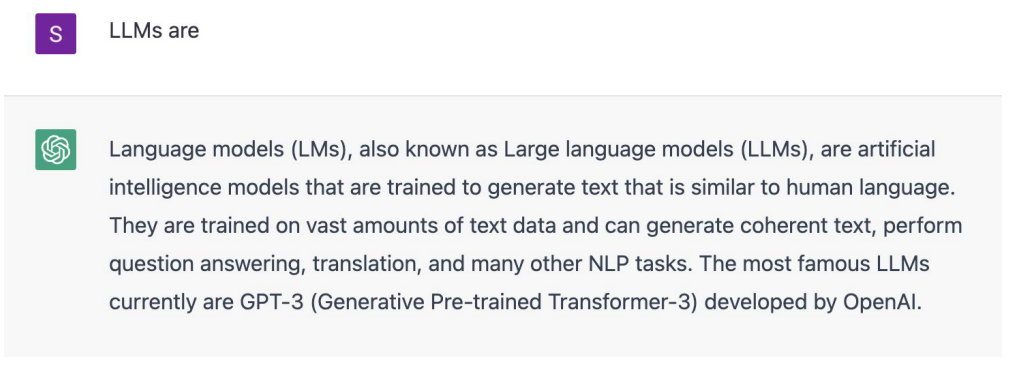
\includegraphics[width=\linewidth,keepaspectratio]{promptengg10}

{\tiny (Ref: Prompt Engineering Sudalai Rajkumar)}

\end{center}		
		


\end{frame}

%%%%%%%%%%%%%%%%%%%%%%%%%%%%%%%%%%%%%%%%%%%%%%%%%%%%%%%%%%%
\begin{frame}[fragile]\frametitle{Text Classification}

\begin{center}
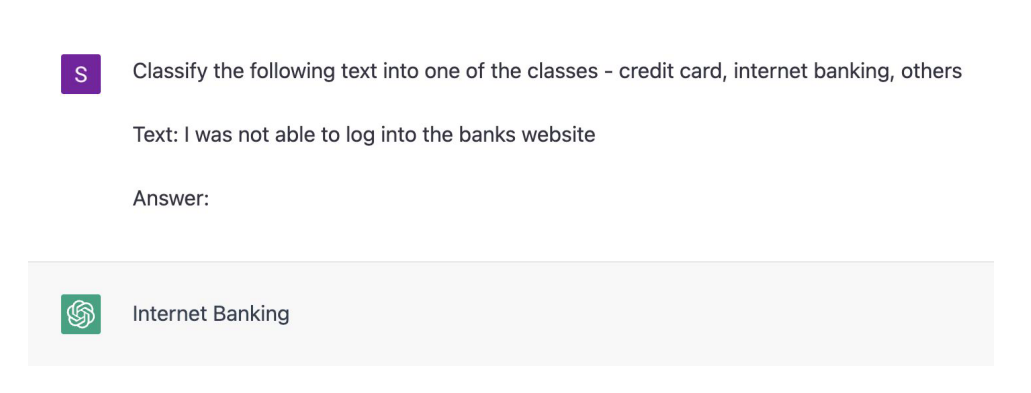
\includegraphics[width=\linewidth,keepaspectratio]{promptengg11}

{\tiny (Ref: Prompt Engineering Sudalai Rajkumar)}

\end{center}		
		


\end{frame}

%%%%%%%%%%%%%%%%%%%%%%%%%%%%%%%%%%%%%%%%%%%%%%%%%%%%%%%%%%%
\begin{frame}[fragile]\frametitle{Text Translation}

\begin{center}

\includegraphics[width=\linewidth,keepaspectratio]{promptengg12}

{\tiny (Ref: Prompt Engineering Sudalai Rajkumar)}

\end{center}		
		


\end{frame}

%%%%%%%%%%%%%%%%%%%%%%%%%%%%%%%%%%%%%%%%%%%%%%%%%%%%%%%%%%%
\begin{frame}[fragile]\frametitle{Text Comprehension}

\begin{center}
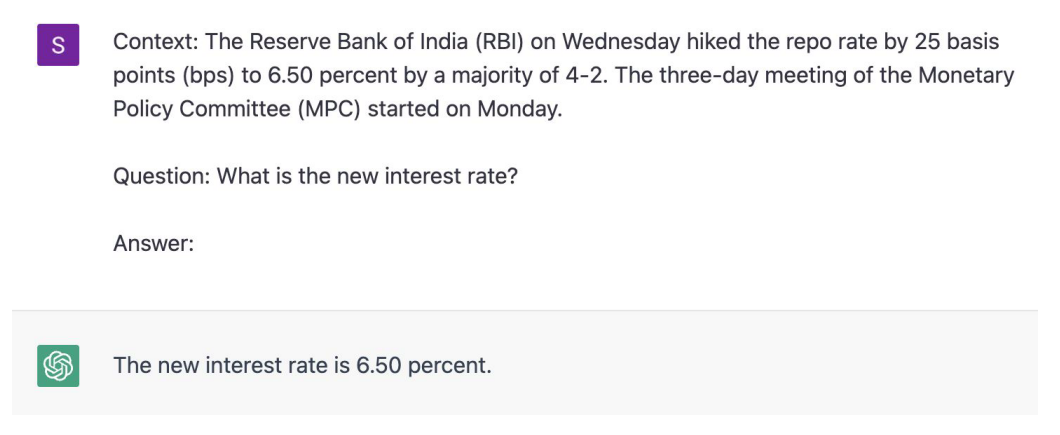
\includegraphics[width=\linewidth,keepaspectratio]{promptengg13}

{\tiny (Ref: Prompt Engineering Sudalai Rajkumar)}

\end{center}		
		


\end{frame}

%%%%%%%%%%%%%%%%%%%%%%%%%%%%%%%%%%%%%%%%%%%%%%%%%%%%%%%%%%%
\begin{frame}[fragile]\frametitle{Text Summarization}

\begin{center}
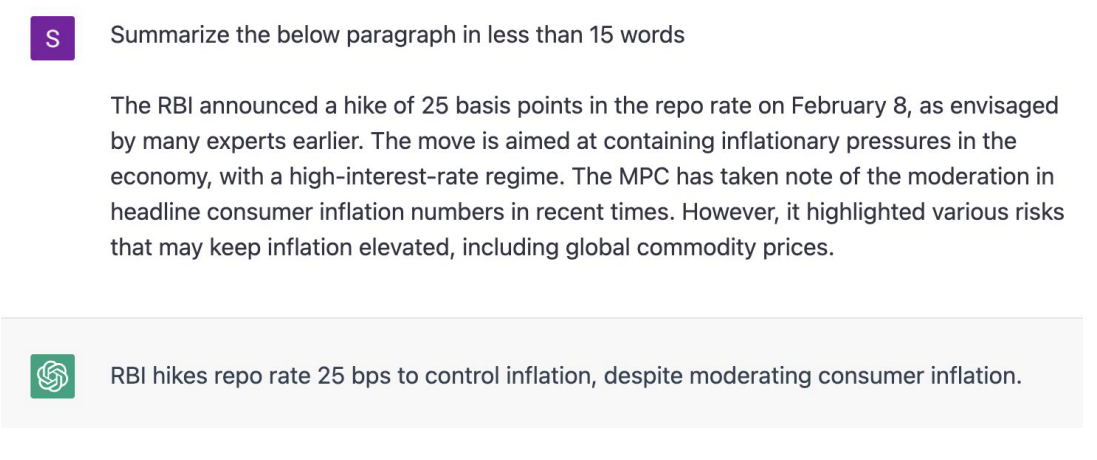
\includegraphics[width=\linewidth,keepaspectratio]{promptengg14}

{\tiny (Ref: Prompt Engineering Sudalai Rajkumar)}

\end{center}		
		


\end{frame}


%%%%%%%%%%%%%%%%%%%%%%%%%%%%%%%%%%%%%%%%%%%%%%%%%%%%%%%%%%%
\begin{frame}[fragile]\frametitle{Question Answering}

\begin{center}
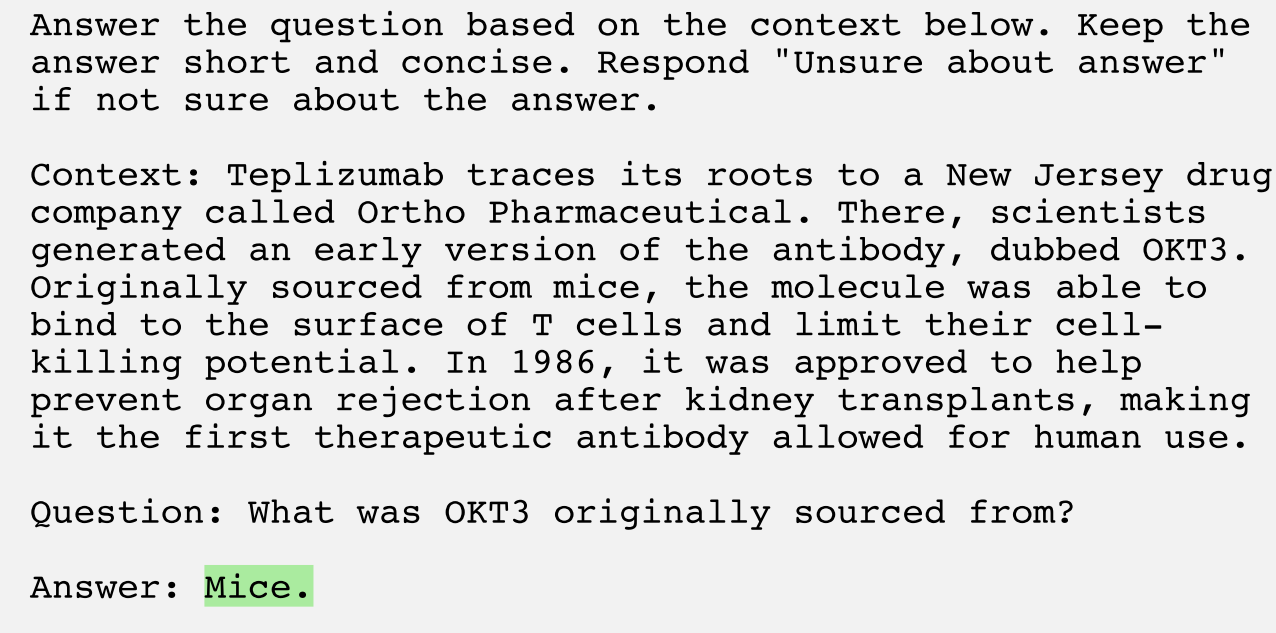
\includegraphics[width=\linewidth,keepaspectratio]{promptengg43}

{\tiny (Ref: Prompt Engineering A lecture by DAIR.AI)}

\end{center}
\end{frame}


%%%%%%%%%%%%%%%%%%%%%%%%%%%%%%%%%%%%%%%%%%%%%%%%%%%%%%%%%%%
\begin{frame}[fragile]\frametitle{Role Playing}

\begin{center}
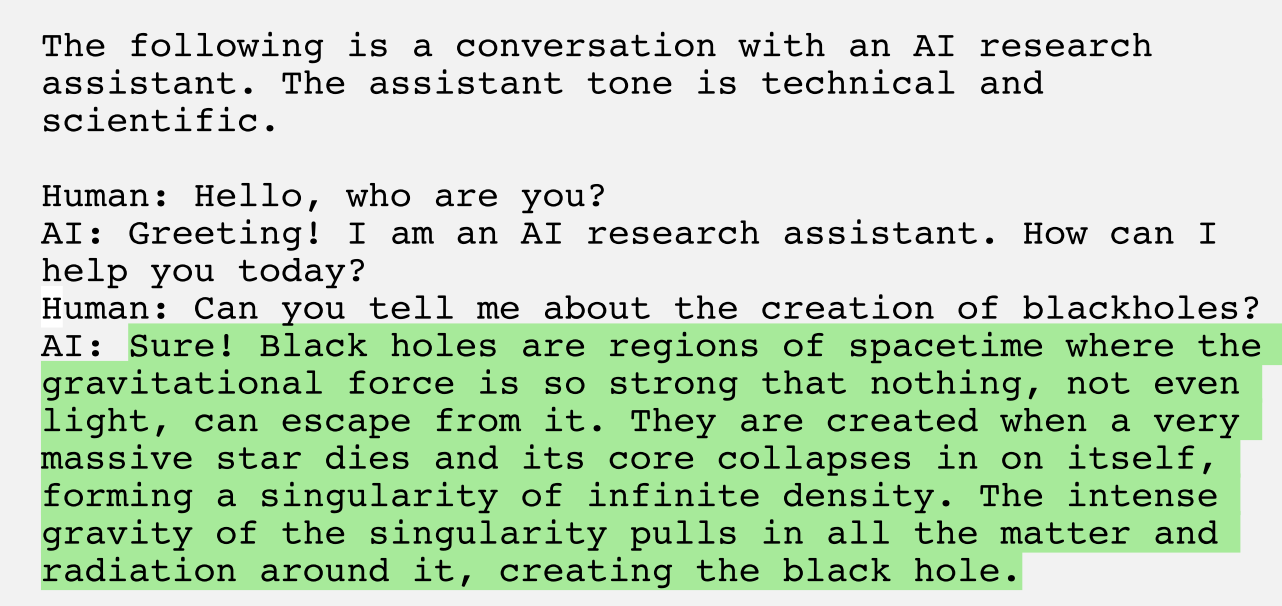
\includegraphics[width=\linewidth,keepaspectratio]{promptengg44}

{\tiny (Ref: Prompt Engineering A lecture by DAIR.AI)}

\end{center}
\end{frame}


%%%%%%%%%%%%%%%%%%%%%%%%%%%%%%%%%%%%%%%%%%%%%%%%%%%%%%%%%%%
\begin{frame}[fragile]\frametitle{Image Generation}

\begin{center}
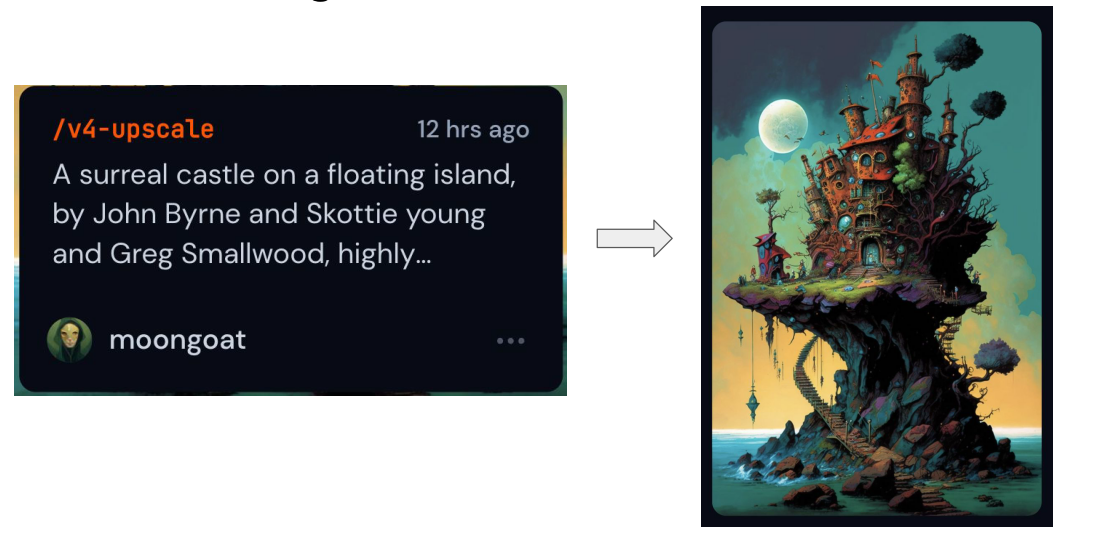
\includegraphics[width=\linewidth,keepaspectratio]{promptengg15}

{\tiny (Ref: Prompt Engineering Sudalai Rajkumar)}

\end{center}		
		
		
Models / Tools: Dall-E , Midjourney, Stable Diffusion

\end{frame}

%%%%%%%%%%%%%%%%%%%%%%%%%%%%%%%%%%%%%%%%%%%%%%%%%%%%%%%%%%%
\begin{frame}[fragile]\frametitle{Prompting Midjourney}


\begin{columns}
    \begin{column}[T]{0.6\linewidth}
		\begin{center}
		
\includegraphics[width=\linewidth,keepaspectratio]{promptengg67}

		{\tiny (Ref: The Complete Prompt Engineering for AI Bootcamp (2023))}
		\end{center}	
    \end{column}
    \begin{column}[T]{0.4\linewidth}
		This is a simple prompt we can use with Midjourney when generating a stock photo of a business meeting.
    \end{column}
  \end{columns}
\end{frame}

%%%%%%%%%%%%%%%%%%%%%%%%%%%%%%%%%%%%%%%%%%%%%%%%%%%%%%%%%%%
\begin{frame}[fragile]\frametitle{Providing Examples to Midjourney}


\begin{columns}
    \begin{column}[T]{0.6\linewidth}
		\begin{center}
		
\includegraphics[width=\linewidth,keepaspectratio]{promptengg68}

		{\tiny (Ref: The Complete Prompt Engineering for AI Bootcamp (2023))}
		\end{center}	
    \end{column}
    \begin{column}[T]{0.4\linewidth}
		Providing examples in your prompts improves the reliability of your output.
		Transform the base image with the words in the prompt to make it your own.
    \end{column}
  \end{columns}
\end{frame}

%%%%%%%%%%%%%%%%%%%%%%%%%%%%%%%%%%%%%%%%%%%%%%%%%%%%%%%%%%%
\begin{frame}[fragile]\frametitle{Giving Direction to Midjourney}


\begin{columns}
    \begin{column}[T]{0.6\linewidth}
		\begin{center}
		
\includegraphics[width=\linewidth,keepaspectratio]{promptengg70}

		{\tiny (Ref: The Complete Prompt Engineering for AI Bootcamp (2023))}
		\end{center}	
    \end{column}
    \begin{column}[T]{0.4\linewidth}
		Describing what you’re imagining, gets you output that matches your vision.
		Transform the base image with the words in the prompt to make it your own.
    \end{column}
  \end{columns}
\end{frame}

%%%%%%%%%%%%%%%%%%%%%%%%%%%%%%%%%%%%%%%%%%%%%%%%%%%%%%%%%%%
\begin{frame}[fragile]\frametitle{Formatting Responses to Midjourney}


\begin{columns}
    \begin{column}[T]{0.6\linewidth}
		\begin{center}
		
\includegraphics[width=\linewidth,keepaspectratio]{promptengg72}

		{\tiny (Ref: The Complete Prompt Engineering for AI Bootcamp (2023))}
		\end{center}	
    \end{column}
    \begin{column}[T]{0.4\linewidth}
		Demonstrating your required response format, minimizes time spent parsing errors. 
		Use formats that are well-recognized and likely to appear in training data.
    \end{column}
  \end{columns}
\end{frame}

%%%%%%%%%%%%%%%%%%%%%%%%%%%%%%%%%%%%%%%%%%%%%%%%%%%%%%%%%%%
\begin{frame}[fragile]\frametitle{Evaluating Quality to Midjourney}


\begin{columns}
    \begin{column}[T]{0.6\linewidth}
		\begin{center}
		
\includegraphics[width=\linewidth,keepaspectratio]{promptengg74}

		{\tiny (Ref: The Complete Prompt Engineering for AI Bootcamp (2023))}
		\end{center}	
    \end{column}
    \begin{column}[T]{0.4\linewidth}
		Test prompts to iterate and improve on the reliability of your results.
		Try different combinations systematically to identify where it fails and succeeds.
    \end{column}
  \end{columns}
\end{frame}

%%%%%%%%%%%%%%%%%%%%%%%%%%%%%%%%%%%%%%%%%%%%%%%%%%%%%%%%%%%
\begin{frame}[fragile]\frametitle{Chaining AIs to Midjourney}


\begin{columns}
    \begin{column}[T]{0.6\linewidth}
		\begin{center}
		
\includegraphics[width=\linewidth,keepaspectratio]{promptengg76}

		{\tiny (Ref: The Complete Prompt Engineering for AI Bootcamp (2023))}
		\end{center}	
    \end{column}
    \begin{column}[T]{0.4\linewidth}
		Combine multiple AI responses, allows you to complete more complex tasks.
		Special-purpose AIs can serve well for common tasks, and correct the mistakes of general models.
    \end{column}
  \end{columns}
\end{frame}

%%%%%%%%%%%%%%%%%%%%%%%%%%%%%%%%%%%%%%%%%%%%%%%%%%%%%%%%%%%
\begin{frame}[fragile]\frametitle{Code Generation}

\begin{center}
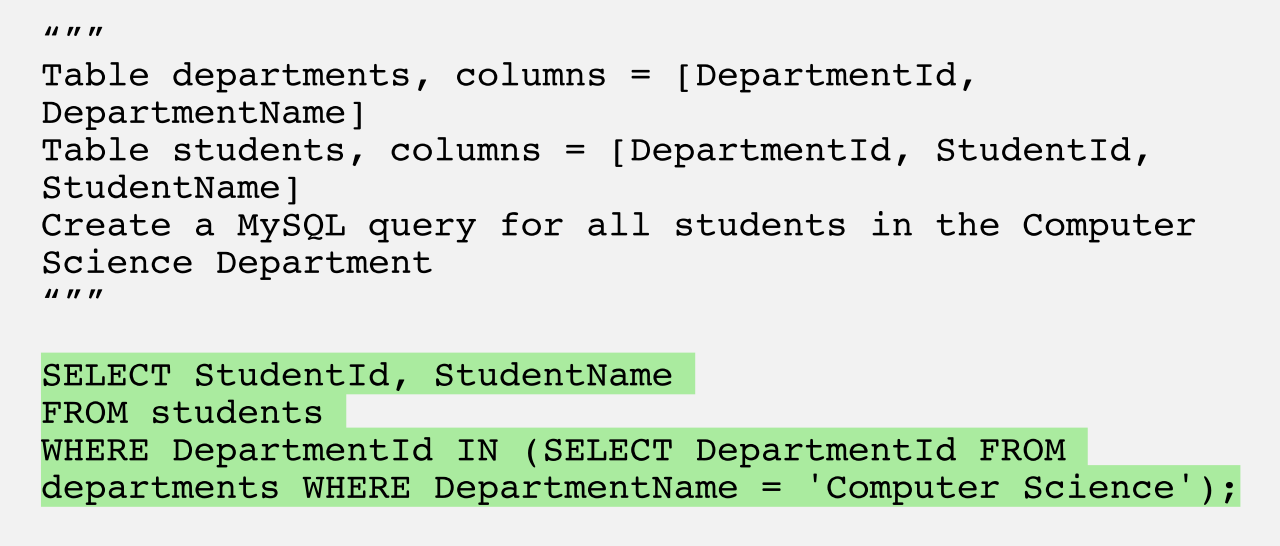
\includegraphics[width=\linewidth,keepaspectratio]{promptengg45}

{\tiny (Ref: Prompt Engineering A lecture by DAIR.AI)}

\end{center}
\end{frame}

%%%%%%%%%%%%%%%%%%%%%%%%%%%%%%%%%%%%%%%%%%%%%%%%%%%%%%%%%%%
\begin{frame}[fragile]\frametitle{Github Co-Pilot}

\begin{columns}
    \begin{column}[T]{0.6\linewidth}
		\begin{center}
		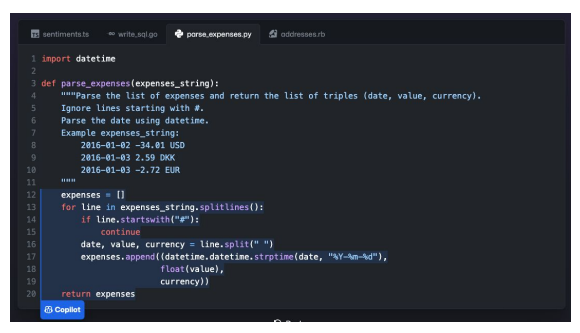
\includegraphics[width=\linewidth,keepaspectratio]{promptengg77}

		{\tiny (Ref: The Complete Prompt Engineering for AI Bootcamp (2023))}
		\end{center}	
    \end{column}
    \begin{column}[T]{0.4\linewidth}
		OpenAI Codex suggests code in real-time, right from your editor. Accessed within a coding
editor called Visual Studio Code
    \end{column}
  \end{columns}
\end{frame}

%%%%%%%%%%%%%%%%%%%%%%%%%%%%%%%%%%%%%%%%%%%%%%%%%%%%%%%%%%%
\begin{frame}[fragile]\frametitle{Github Co-Pilot}

		\begin{center}
		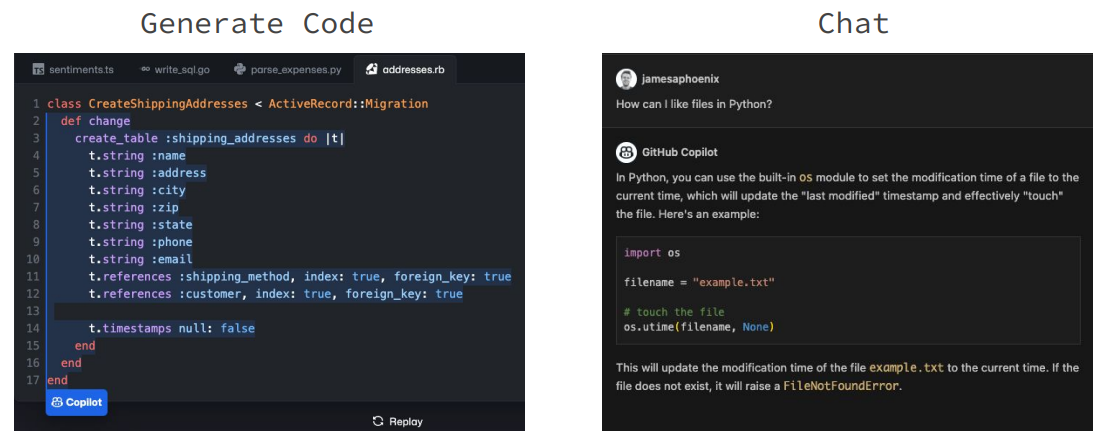
\includegraphics[width=\linewidth,keepaspectratio]{promptengg78}

		{\tiny (Ref: The Complete Prompt Engineering for AI Bootcamp (2023))}
		\end{center}	

\end{frame}

%%%%%%%%%%%%%%%%%%%%%%%%%%%%%%%%%%%%%%%%%%%%%%%%%%%%%%%%%%%
\begin{frame}[fragile]\frametitle{Github Co-Pilot}


\begin{columns}
    \begin{column}[T]{0.6\linewidth}
		\begin{center}
		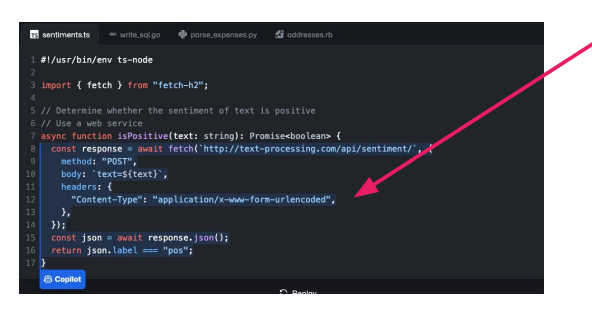
\includegraphics[width=\linewidth,keepaspectratio]{promptengg79}

		{\tiny (Ref: The Complete Prompt Engineering for AI Bootcamp (2023))}
		\end{center}	
    \end{column}
    \begin{column}[T]{0.4\linewidth}
		Github Co-pilot can generate code from comments or function names.
    \end{column}
  \end{columns}
\end{frame}

%%%%%%%%%%%%%%%%%%%%%%%%%%%%%%%%%%%%%%%%%%%%%%%%%%%%%%%%%%%
\begin{frame}[fragile]\frametitle{Github Co-Pilot}


\begin{columns}
    \begin{column}[T]{0.6\linewidth}
		\begin{center}
		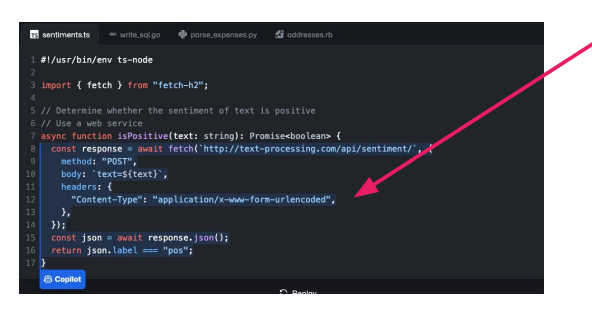
\includegraphics[width=\linewidth,keepaspectratio]{promptengg79}

		{\tiny (Ref: The Complete Prompt Engineering for AI Bootcamp (2023))}
		\end{center}	
    \end{column}
    \begin{column}[T]{0.4\linewidth}
		Co-pilot will parse your project’s code, therefore it can adapt to your coding style and project.
		If you’re not happy with the code output you can change to a new suggestion.
    \end{column}
  \end{columns}
\end{frame}

%%%%%%%%%%%%%%%%%%%%%%%%%%%%%%%%%%%%%%%%%%%%%%%%%%%%%%%%%%%
\begin{frame}[fragile]\frametitle{For generating code using Codex}

Limitations


\begin{itemize}
\item  ChatGPT outputs more extensive code. However Co-pilot’s recommendations are good for whilst being in the flow of
coding.
\item Can be slower as your project size grows.
\item Doesn’t have any model options. The only way we can influence the output is with:
	\begin{itemize}
	\item More extensive comments.
	\item Function/Class names.
	\item The existing code within your project.
	\item Adding types to your code.
	\item Using different packages.
	\end{itemize}	 
\end{itemize}	 

{\tiny (Ref: The Complete Prompt Engineering for AI Bootcamp (2023))}

\end{frame}

%%%%%%%%%%%%%%%%%%%%%%%%%%%%%%%%%%%%%%%%%%%%%%%%%%%%%%%%%%%
\begin{frame}[fragile]\frametitle{Reasoning}

\begin{center}
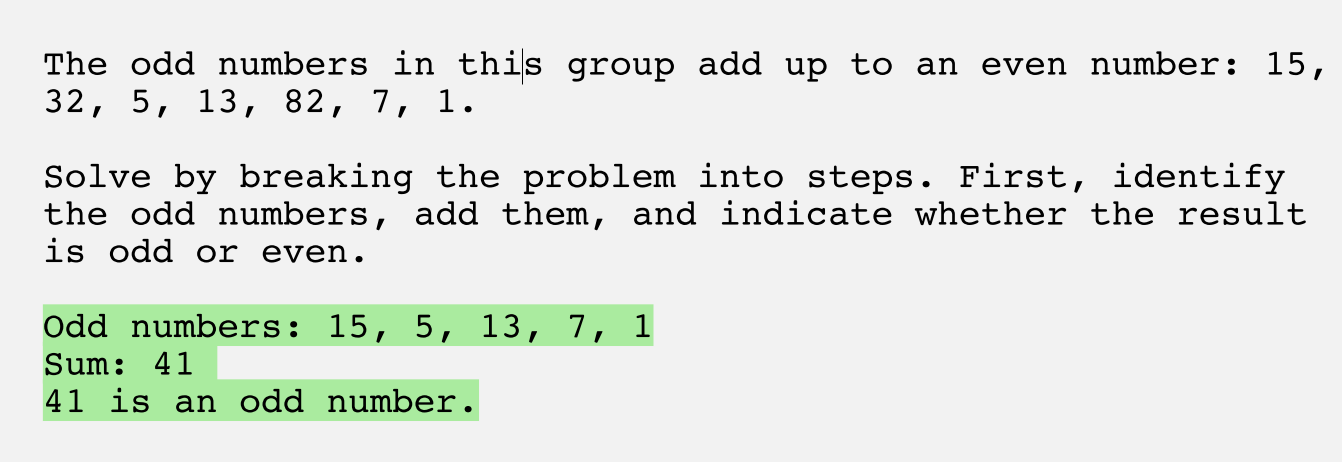
\includegraphics[width=\linewidth,keepaspectratio]{promptengg46}

{\tiny (Ref: Prompt Engineering A lecture by DAIR.AI)}

\end{center}
\end{frame}




%%%%%%%%%%%%%%%%%%%%%%%%%%%%%%%%%%%%%%%%%%%%%%%%%%%%%%%%%%%
\begin{frame}[fragile]\frametitle{For generating code using Codex}

Provide Codex with a prompt consisting of the following:



\begin{itemize}
\item  High level task description: Tell the model to use a helpful tone when outputting natural language
\item  High level context: Describe background information like API hints and database schema to help the model understand the task
\item  Examples: Show the model examples of what you want
\item  User input: Remind the model what the user has said before
\end{itemize}	 

{\tiny (Ref: https://microsoft.github.io/prompt-engineering/)}

\end{frame}

% %%%%%%%%%%%%%%%%%%%%%%%%%%%%%%%%%%%%%%%%%%%%%%%%%%%%%%%%%%%
% \begin{frame}[fragile]\frametitle{For Cypher code For Neo4j}


% Provide examples within prompt:

% {\tiny (Ref:https://github.com/tomasonjo/langchain2neo4j)}

% \begin{lstlisting}
% # Who played in Top Gun?
% MATCH (m:Movie)<-[r:ACTED_IN]-(a)
% RETURN {{actor: a.name, role: r.role}} AS result
% # What is the plot of the Copycat movie?
% MATCH (m:Movie {{title: "Copycat"}})
% RETURN {{plot: m.plot}} AS result
% # Did Luis Guzman appear in any other movies?
% MATCH (p:Person {{name:"Luis Guzman"}})-[r:ACTED_IN]->(movie)
% RETURN {{movie: movie.title, role: r.role}} AS result
% # Do you know of any matrix movies?
% MATCH (m:Movie)
% WHERE toLower(m.title) CONTAINS toLower("matrix")
% RETURN {{movie:m.title}} AS result
% \end{lstlisting}	 


% \end{frame}

% %%%%%%%%%%%%%%%%%%%%%%%%%%%%%%%%%%%%%%%%%%%%%%%%%%%%%%%%%%%
% \begin{frame}[fragile]\frametitle{Crazy ideas}

% \begin{itemize}
% \item Stop asking ChatGPT for information - start an actual conversation.
% “What's the population of Topeka?” Gah! ChatGPT isn't Google. Google is Google. ChatGPT is a brilliant, patient thought partner.
% EXAMPLE: Tell it *why* you want to know about Topeka. “I'm starting a consulting business in Topeka, I have \$20k, two kids in middle school, I studied biology, I worked for McKinsey. What are ten reasons my business might succeed or fail?”
% Feed it more and more detail about your work experience, family, etc. - that's where the magic happens.

% \item Create actual characters to debate your Big Idea before presenting it.
% Test your work ideas on ChatGPT, which will play the roles of colleagues.
% EXAMPLE: Tell ChatGPT “Play 4 roles for me: Be my company's CEO, CMO, CTO, and CFO. (Describe each person- Technical? Fiscally conservative? Passive aggressive?) Probe the following idea for weaknesses.”
% A bit traumatic, right? Okay, Step Two: Tell ChatGPT “Now become a smarter version of all those executives and give counter-arguments as to why my idea is brilliant.”
% Invite historical guests! Ask Steve Jobs to make a case for your idea! Or Einstein!

% \end{itemize}	 

% {\tiny (Ref: LinkedIn post by Dr Joerg Storm)}
			

% \end{frame}

% %%%%%%%%%%%%%%%%%%%%%%%%%%%%%%%%%%%%%%%%%%%%%%%%%%%%%%%%%%%
% \begin{frame}[fragile]\frametitle{Crazy ideas}

% \begin{itemize}

% \item ChatGPT is built for creatives. And it wants ALL the smoke.
% ChatGPT isn't a racehorse - it's freakin' Seabiscuit. It wants to show off. People give up because they pose a general question and get a general answer. Get specific!
% EXAMPLE:
% Don't ask “What are strategies for handling an annoying co-worker?”
% Instead, try “I work in a San Jose crayon factory in quality control. My colleague points out every crayon I've missed and asks gas-lighting questions. What are three indirect ways to stop his behavior and what is one direct thing I can say?” Ask follow up questions.

% \item Talk to it like a trusted, brilliant friend.
% EXAMPLE: You call your brilliant friend and go “Hey Taylor, how does Walmart decide what to stock?” You don't say: “Taylor, give four ways Walmart prioritizes items for display.” Taylor would think you're being held hostage.
% Don't get me wrong - you *can* ask ChatGPT like that. But it undermines your strength - your EQ. Relax and talk to it like a friend. It will unlock your creativity.

% \item Don't stop after your Crappy First Draft.
% Writing is rewriting. Remember your college professor shouting that? ChatGPT will give different results as you tweak the wording. ChatGPT loves this stuff.
% EXAMPLE: Different words elicit different responses. Try new command words, new adjectives, verb choices. Try more detail. (This is basically prompt engineering.) Don't give up! Did 4 years at Vassar teach you nothing?
% \end{itemize}	 

% {\tiny (Ref: LinkedIn post by Dr Joerg Storm)}
			

% \end{frame}


% %%%%%%%%%%%%%%%%%%%%%%%%%%%%%%%%%%%%%%%%%%%%%%%%%%%%%%%%%%%
% \begin{frame}[fragile]\frametitle{Crazy ideas}

% \begin{itemize}
% \item Have it create its own prompt
% If you’re trying out a new topic or not getting the results you want, turn ChatGPT into its own helper. Say, ''I want to create a new marketing plan for the year for my new golf brand. Tell me what information you need to create the best plan, and write a prompt my team and I can use in the future for similar requests.”
% \item Create an AI prompt for your brand
% Today’s brand guidelines already have colors, logo usage, and design lockups - adding an AI prompt for your brand voice. Grab a bunch of branded copy from your website, ads, and blogs. Submit it to ChatGPT and ask the system to describe that writing to be used later as brand guidelines for your whole company. Test and iterate until you’re happy with it. Then have a shared prompt for your team, like: ''We are \ldots, we build \ldots for \ldots, and for all writing I ask you to complete, please write it in the following style: \ldots''. This creates an even more consistent brand voice!
% \item Personalize it to you and only you
% Most people I talk with don’t add enough parameters to their prompts, resulting in extremely generic, low-quality outputs. Add in more restrictions. Don’t just say: ''Create a 5-day travel itinerary for Lisbon.” Instead, say, ''Create an hour-by-hour 5-day travel itinerary for Lisbon. Keep in mind, I am a 45-year-old male, traveling alone. I hate golf, spinach, and wind. I love archery, farm animals, coffee, and horror films. I like temperatures over 65 degrees, I want to spend less than \$500 a day, and I want to see at least two sunsets from viewpoints.”
% \end{itemize}	 

% {\tiny (Ref: LinkedIn post by Allie K Miller)}
			

% \end{frame}

% %%%%%%%%%%%%%%%%%%%%%%%%%%%%%%%%%%%%%%%%%%%%%%%%%%%%%%%%%%%
% \begin{frame}[fragile]\frametitle{Crazy ideas}

% \begin{itemize}
% \item Play fill in the blank
% Treat it like reverse Madlibs. If you’re stuck on a writing section or phrase or word, just replace it with a variable (like ''XK”) and ask the system to fill in the blank whenever it sees that variable. Overcoming writer’s block is a great use case.
% \item Hone your debate
% The ability to influence is a superpower in business. Try out ChatGPT as a sparring partner for upcoming debates or decisions. Give it a topic or argument, then ask the system to take a position either for or against it. Engage in a back-and-forth dialogue, refining your points and counterpoints, to develop more persuasive arguments and improve your critical thinking skills.
% \item Use variables like a menu
% Embed several sub-prompts and parameter options, like a restaurant menu. ''I will give you an <ask>, a <voice>, and an <output style>. Voices options are: 1 - funny and irreverent in the style of Jerry Seinfeld, 2 - formal and academic in the style of James Carville, etc. Output style options are: 1 - text, 2 - table, 3 - decision tree, 4 - ascii drawing, etc.” Make these LONG and SPECIFIC. That way, when I prompt ChatGPT, I just pick from my menu and write: ''Ask = research on stingrays, voice = 8, output style = 3”. This is a massive timesaver!
% \end{itemize}	 

% {\tiny (Ref: LinkedIn post by Allie K Miller)}
			

% \end{frame}


%%%%%%%%%%%%%%%%%%%%%%%%%%%%%%%%%%%%%%%%%%%%%%%%%%%%%%%%%%%%%%%%%%%%%%%%%%%%%%%%%%
\begin{frame}[fragile]\frametitle{}
\begin{center}
{\Large Prompts for Business and Life}
\end{center}

{\tiny (Ref: LinkedIn post by Zain Kahn)}
\end{frame}

%%%%%%%%%%%%%%%%%%%%%%%%%%%%%%%%%%%%%%%%%%%%%%%%%%%%%%%%%%%%%%%%%%%%%%%%%%%%%%%%%%
\begin{frame}[fragile]\frametitle{ChatGPT Mental Model Prompts}
\textbf{1. First Principles Thinking}
\begin{itemize}
    \item Use First Principles to evaluate [insert your decision].
    \item List underlying assumptions affecting this decision.
\end{itemize}
\end{frame}

%%%%%%%%%%%%%%%%%%%%%%%%%%%%%%%%%%%%%%%%%%%%%%%%%%%%%%%%%%%%%%%%%%%%%%%%%%%%%%%%%%
\begin{frame}[fragile]\frametitle{ChatGPT Mental Model Prompts (contd.)}
\textbf{2. Occam's Razor}
\begin{itemize}
    \item Provide simple explanation for good/bad decision.
    \item Apply to [insert decision].
\end{itemize}

\textbf{3. Enhance Problem Solving}
\begin{itemize}
    \item [insert problem]
    \item Step-by-step solution with clear instructions.
\end{itemize}
\end{frame}

%%%%%%%%%%%%%%%%%%%%%%%%%%%%%%%%%%%%%%%%%%%%%%%%%%%%%%%%%%%%%%%%%%%%%%%%%%%%%%%%%%
\begin{frame}[fragile]\frametitle{ChatGPT Mental Model Prompts (contd.)}
\textbf{4. Pros and Cons}
\begin{itemize}
    \item Decide [insert decision].
    \item List pros and cons for clarity.
\end{itemize}

\textbf{5. The 80/20 Method}
\begin{itemize}
    \item Identify key factors, 20% that affect 80% benefit.
    \item Apply to [insert decision].
\end{itemize}
\end{frame}

%%%%%%%%%%%%%%%%%%%%%%%%%%%%%%%%%%%%%%%%%%%%%%%%%%%%%%%%%%%%%%%%%%%%%%%%%%%%%%%%%%
\begin{frame}[fragile]\frametitle{ChatGPT Mental Model Prompts (contd.)}
\textbf{6. Get Feedback from Famous Minds}
\begin{itemize}
    \item Assume [insert famous person, e.g. Steve Jobs].
    \item Read decision, provide feedback as [insert person].
\end{itemize}

\textbf{7. Systems Thinking}
\begin{itemize}
    \item Analyze decision as part of larger system.
    \item Identify key variables affecting wider system.
\end{itemize}
\end{frame}

%%%%%%%%%%%%%%%%%%%%%%%%%%%%%%%%%%%%%%%%%%%%%%%%%%%%%%%%%%%%%%%%%%%%%%%%%%%%%%%%%%
\begin{frame}[fragile]\frametitle{ChatGPT Mental Model Prompts (contd.)}
\textbf{8. Second Order Effects}
\begin{itemize}
    \item List second order effects due to decision.
    \item Apply to [insert decision].
\end{itemize}

\textbf{9. Regret Minimization Framework}
\begin{itemize}
    \item Consider regrets for [insert decision].
    \item List alternate decisions to reduce regret.
\end{itemize}
\end{frame}

%%%%%%%%%%%%%%%%%%%%%%%%%%%%%%%%%%%%%%%%%%%%%%%%%%%%%%%%%%%%%%%%%%%%%%%%%%%%%%%%%%
\begin{frame}[fragile]\frametitle{ChatGPT Mental Model Prompts (contd.)}
\textbf{10. Opportunity Cost}
\begin{itemize}
    \item Evaluate decision's opportunity cost.
    \item List alternate opportunities foregone.
\end{itemize}
\end{frame}